\documentclass[11pt,border=0mm,tikz]{standalone}
\usepackage{csquotes}
\usepackage[backend=biber,style=numeric,sorting=none]{biblatex}

\providecommand{\FigScale}{1}

\usepackage{siunitx}
\usepackage{tikz}
\usetikzlibrary{decorations.pathmorphing,patterns}
\usetikzlibrary{shapes.geometric, arrows.meta}
\usetikzlibrary{positioning}
\usepackage{amsmath}
\usepackage{upgreek}
\usepackage{svg}
\usetikzlibrary{3d}
\usetikzlibrary{calc}
\tikzset{
box/.style={
	rectangle,
	rounded corners=4pt,
	minimum width=3cm,
	minimum height=1cm,
	text centered,
    align=center,
	draw=black!70,
	line width=0.95pt,
	fill=gray!5,
	inner sep=4pt
},
decision/.style={
	diamond,
	aspect=2,
	text centered,
	align=center,
	draw=black!70,
	line width=0.95pt,
	fill=gray!5,
	inner sep=1pt
},
arrow/.style={
	thick,
	->,
	>=Stealth,
	draw=black!70,
	line width=1pt,
	line cap=round,
	line join=round,
	shorten <=1pt,
	shorten >=1pt
}
}
\begin{document}
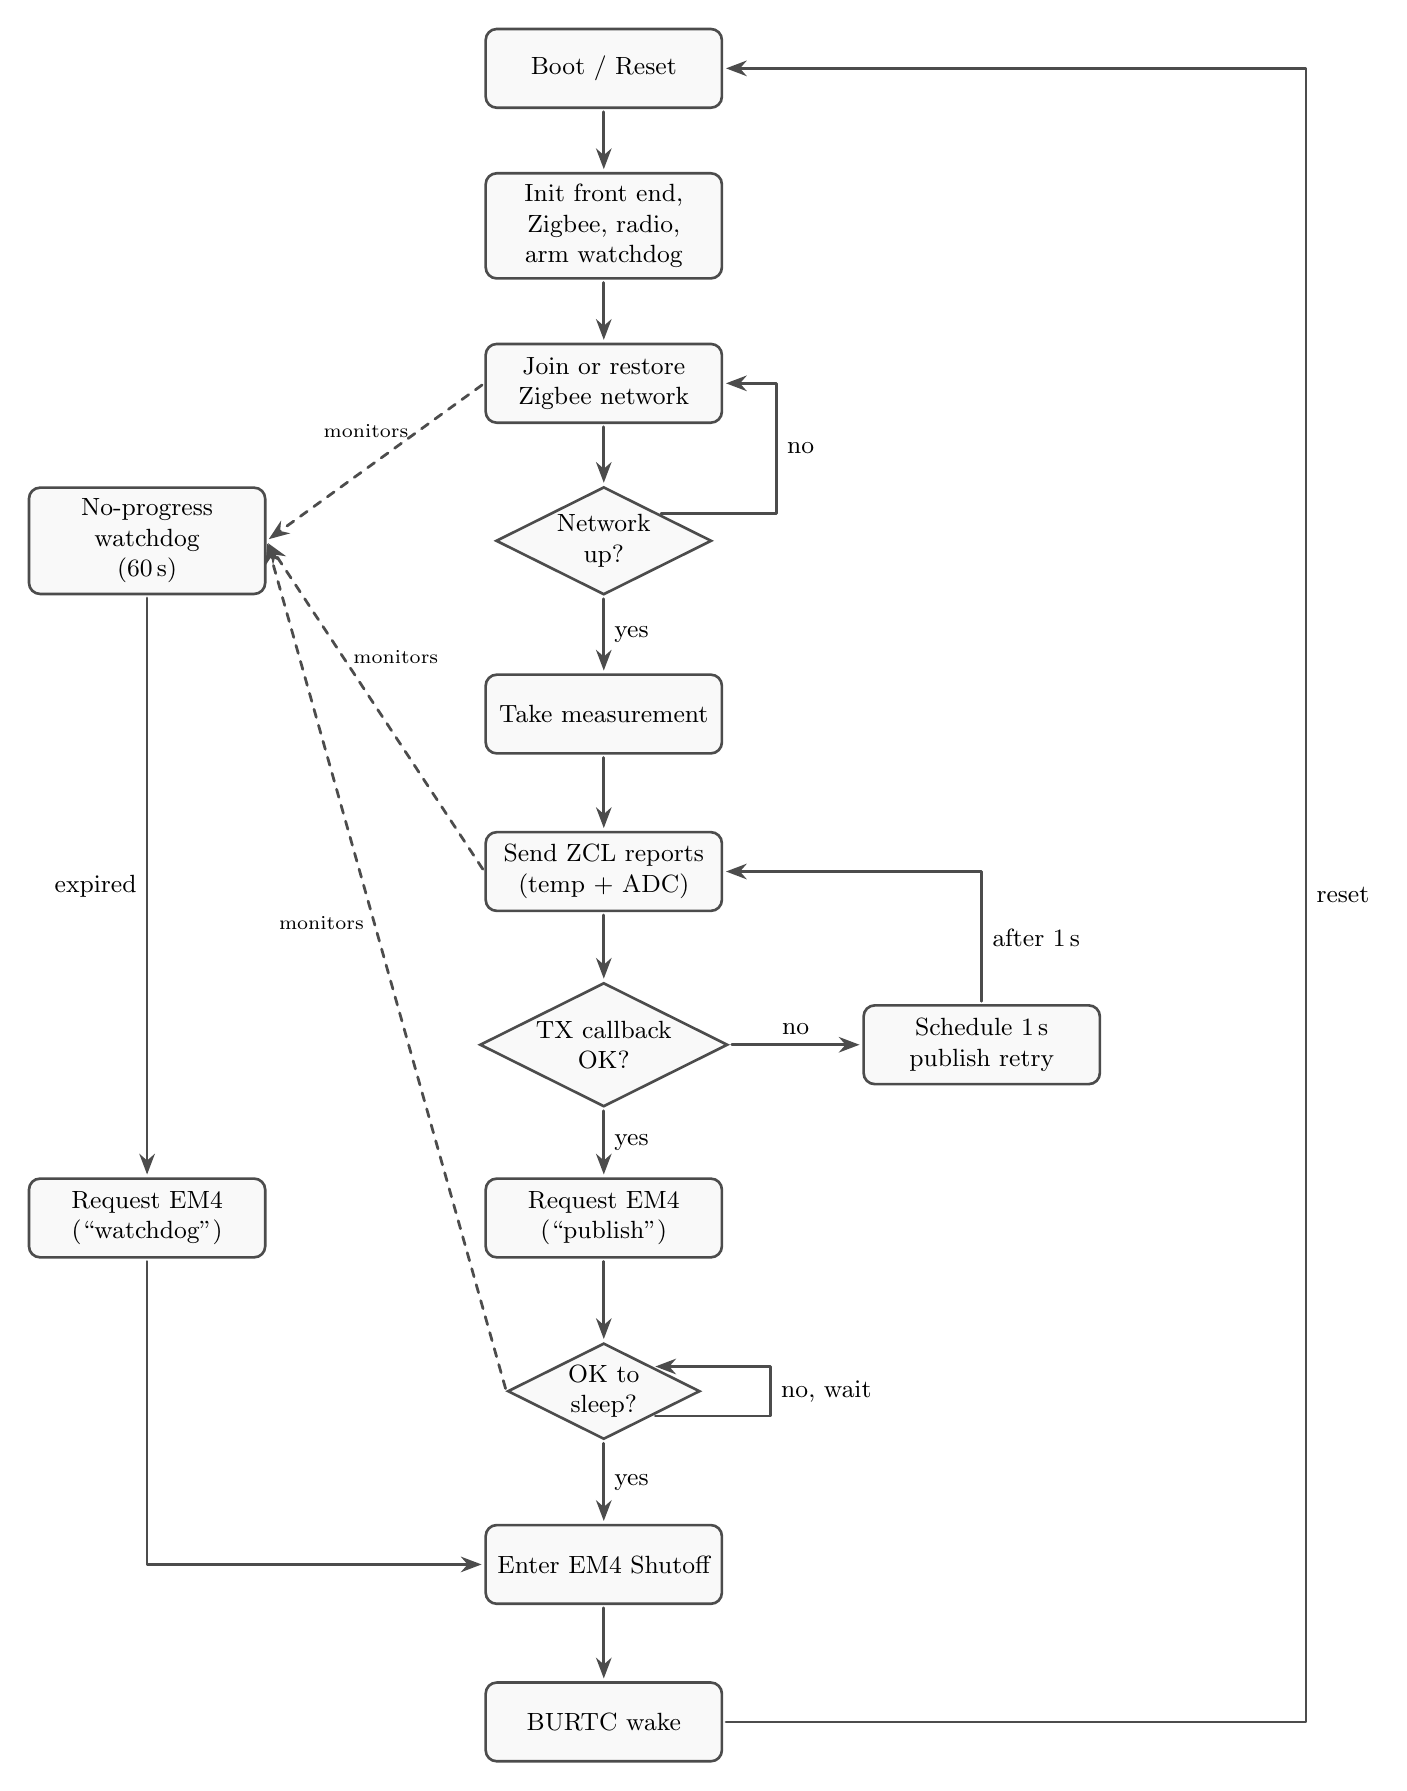
\begin{tikzpicture}[scale=\FigScale, font=\small]
% ===== Main vertical happy path (centre column, x = 0) =====
\node (boot)    [box]                         at (0, 0)    {Boot / Reset};
\node (init)    [box]                         at (0, -2)   {Init front end,\\Zigbee, radio,\\arm watchdog};
\node (join)    [box]                         at (0, -4)   {Join or restore\\Zigbee network};
\node (upq)     [decision]                    at (0, -6)   {Network\\up?};
\node (measure) [box]                         at (0, -8.2) {Take measurement};
\node (report)  [box]                         at (0, -10.2){Send ZCL reports\\(temp + ADC)};
\node (txq)     [decision]                    at (0, -12.4){TX callback\\OK?};
\node (em4req)  [box]                         at (0, -14.6){Request EM4\\(``publish'')};
\node (okq)     [decision]                    at (0, -16.8){OK to\\sleep?};
\node (em4)     [box]                         at (0, -19.0){Enter EM4 Shutoff};
\node (wake)    [box]                         at (0, -21.0){BURTC wake};
% ===== Side nodes =====
% TX failure -> retry (right side)
\node (retry)   [box]                         at (4.8, -12.4){Schedule 1\,s\\publish retry};
% Watchdog (left side)
\node (wdog)    [box]                         at (-5.8, -6) {No-progress\\watchdog\\(60\,s)};
\node (em4w)    [box]                         at (-5.8, -14.6){Request EM4\\(``watchdog'')};
% ===== Happy-path arrows =====
\draw [arrow] (boot)    -- (init);
\draw [arrow] (init)    -- (join);
\draw [arrow] (join)    -- (upq);
\draw [arrow] (upq)     -- node[right] {yes} (measure);
\draw [arrow] (measure) -- (report);
\draw [arrow] (report)  -- (txq);
\draw [arrow] (txq)     -- node[right] {yes} (em4req);
\draw [arrow] (em4req)  -- (okq);
\draw [arrow] (okq)     -- node[right] {yes} (em4);
\draw [arrow] (em4)     -- (wake);

% wake -> boot (full reset), routed on the far right
\draw [arrow] (wake.east) -- ++(7.4,0) |- node[pos=0.25, right] {reset} (boot.east);
% Network not up: wait (loop back into join from the right side)
\draw [arrow] (upq.north east) -- ++(1.5,0.0) |- node[pos=0.25, right] {no} (join.east);
% OK to sleep? no -> wait (small loop back into the decision)
\draw [arrow] (okq.south east) -- ++(1.5,0.0) |- node[pos=0.25, right] {no, wait} (okq.north east);
% TX failure -> retry -> back to report after 1 s
\draw [arrow] (txq.east)   -- node[above] {no} (retry.west);
\draw [arrow] (retry.north) |- node[pos=0.25, right] {after 1\,s} (report.east);
% Watchdog: stuck anywhere in active phase -> request EM4 (watchdog) -> EM4
\draw [arrow] (wdog) -- node[left] {expired} (em4w);
\draw [arrow] (em4w.south) |- (em4.west);

% Dashed: the watchdog monitors the whole active phase (join through TX).
\draw [arrow, dashed] (join.west)   -- node[pos=0.3, left, font=\scriptsize] {monitors} (wdog.east);
\draw [arrow, dashed] (report.west) -- node[pos=0.65, right, font=\scriptsize] {monitors} (wdog.east);
\draw [arrow, dashed] (okq.west) -- node[pos=0.55, left, font=\scriptsize] {monitors} (wdog.east);

\end{tikzpicture}
\end{document}